
\documentclass[english]{article}

\usepackage{graphicx}
\usepackage{alltt}
\usepackage{url}
\usepackage{tabularx}
%\usepackage{ngerman}
\usepackage{longtable}
\usepackage{color}
\usepackage{scrextend}

\usepackage{xifthen}
\newboolean{showbackdoors}
\setboolean{showbackdoors}{true}  % set to false to hide subsection on backdoors for reviewing group


\newenvironment{prettytablex}[1]{\vspace{0.3cm}\noindent\tabularx{\linewidth}{@{\hspace{\parindent}}#1@{}}}{\endtabularx\vspace{0.3cm}}
\newenvironment{prettytable}{\prettytablex{l X}}{\endprettytablex}


\title{\huge\sffamily\bfseries System Description and Risk Analysis}
\author{Cyrill Kr\"ahenb\"uhl \and Silvan Egli \and Lukas Bischofberger}
\date{\today}



\begin{document}
\maketitle

%% **** please observe the page limit **** 
%% (it is not allowed to change the font size or page geometry to gain more space)
%% comment or remove lines below before hand-in
%\begin{center}
%{\large\textcolor{red}{Page limit: 30 pages.}}
%\end{center}
%%%%%%%%%%%%%%%%%%%%%%%%%%%%%%%%%%%%%%%%%%%%%%

\tableofcontents
\pagebreak


\section{System Characterization}

\subsection{System Overview}

%%20 points

\begin{figure}[ht]
	\centering
	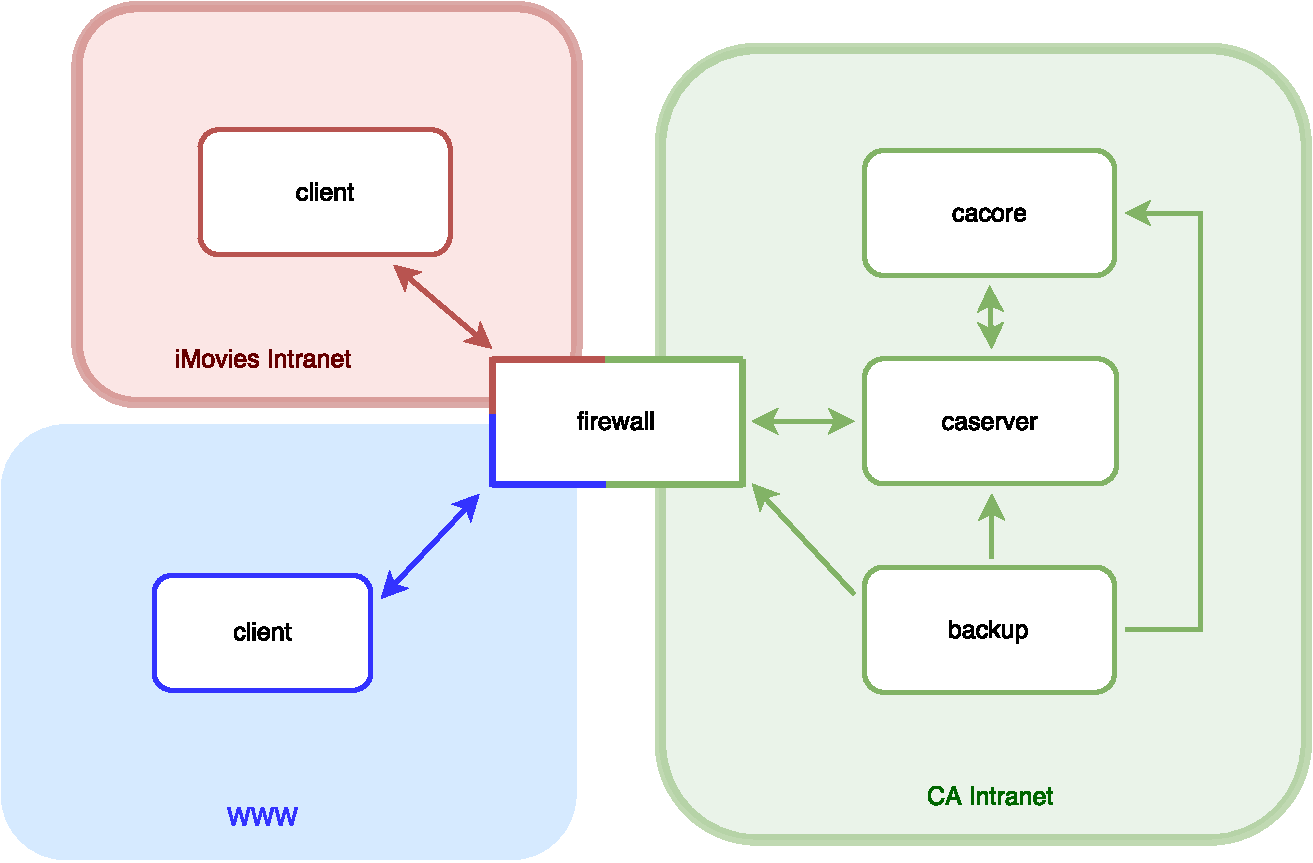
\includegraphics[scale=0.5]{src/systemoverview.pdf}
	\caption{System overview}
	\label{figure:systemoverview}
\end{figure}

The mission of the system consist of providing a certificate authority (CA) service through which employees of the fictional company iMovies can request and revoke digital certificates. These certificates will be used for secure e-mail communication between employees. In the following these employees will be referred to as clients and users.\\
Figure {\ref{figure:systemoverview}} shows an overview of the proposed system. It consist of four subsystems, namely firewall, caserver, cacore and backup and forms the CA Intranet. Clients either use the service from inside the company's network or from the Internet. They are interfaced with the system by the firewall which blocks unallowed connections and forwards the request to the caserver. The caserver subsystem provides a web interface for clients and administrators. It performs the authentication and authorization and handles the user requests as well as their sessions. In order to do so, the caserver makes use of the cacore's service. The cacore's task is to control the process of issuing and revoking certificates as well as managing the user data. The backup is responsible for maintaining a copy of all system relevant data, including information on users, certificates, keys, logs and configurations. Therefore the backup has access to the other three subsystems.

%Describe the system's mission,  the system boundaries,
%and the overall system architecture, including the main subsystems and
%their relationships.   This description should provide a high-level
%overview of the system, e.g., suitable for managers, that complements
%the more technical description that follows.


\subsection{System Functionality} 
 %Describe the system’s functions. 
 % TODO : remove https://en.wikipedia.org/wiki/Functional_requirement
 % https://en.wikipedia.org/wiki/Functional_specification
 In this section we describe the systems functions in terms of system design based on the use cases given in the project assignment. The focus lies on the implementation and the information flows. In subsection \ref{components} the properties of the mentioned applications will be described in more detail.
 
 \subsubsection{Components}\label{compfunc}
 \paragraph{client} 
 Clients use the system through a web interface which is built using the  Angular2\footnote{\url{https://angular.io/}} framework written in TypeScript\footnote{\url{https://www.typescriptlang.org/}}. The web front end consumes the RESTful\footnote{\label{restful}\url{https://en.wikipedia.org/wiki/Representational_state_transfer}} service provided by the back end on the caserver by performing http requests to the firewall. 
 
 \paragraph{firewall}
 In order to block connection attempts to unallowed ports the firewall makes use of the iptables\footnote{\url{http://ipset.netfilter.org/iptables.man.html}} functionality. In addition to the packet filtering, iptables is configured to act as a NAT and thus forwarding requests from the internet and the company's intranet to the web server on the caserver. In order to configure iptables the csf\footnote{\url{https://configserver.com/cp/csf.html}} application is used.
 
 \paragraph{caserver}
The nginx\footnote{\url{https://nginx.org/}} webserver is responsible for handling the forwarded requests from the firewall. This includes delivering static content (front end and certificate revocation list) and forwarding the other requests to the back end. In addition it checks if the client sent a user certificate and verifies it using the root certificate. \\The back end consist of a Django\footnote{\label{django}\url{https://www.djangoproject.com/}} application written in python which is served by a uwsgi\footnote{\url{https://uwsgi-docs.readthedocs.io/en/latest/}} application server  The following tasks are subject to the backend: 

\begin{itemize}
\item user authentication
\item authorization checks
\item session management
\item user input validation
\item output sanitization
\item database queries
\item site calls to the cacore subsystem
\item providing the CA administrator interface
\item providing a RESTful\footref{restful} API to the front end
\end{itemize}

\paragraph{cacore}
On the cacore there is a MySQL\footnote{\url{https://www.mysql.com/}} database containing the legacy user data table and all tables needed by the Django application. The caserver accesses the database over the network. In addition, the cacore provides the functionality of a CA by using the openSSL\footnote{\label{openssl}\url{https://www.openssl.org/}} library.
There is an intermediate CA and a root CA on the cacore. The intermediate CA is used for issuing the user certificates. It's private key is not encrypted in order to sign the user certificates non interactively. The root CA's only task was to issue and sign the intermediate CA's certificate. It's private key is encrypted and kept offline. From now on, when speaking of the CA, the intermediate CA is referenced if not stated otherwise.
The CA supports the creation of new X509\footnote{\url{https://en.wikipedia.org/wiki/X.509}} user certificates as well as their revocation by using the "ca" command of openSSL\footref{openssl}. The certificate creation and revocation are implemented as a Bash\footnote{\url{https://www.gnu.org/software/bash/bash.html}} script which are called by the Django\footref{django} application using ssh\footnote{label{ssh}\url{https://en.wikipedia.org/wiki/Secure_Shell}}.

\paragraph{backup} 

The backup periodically (once every hour) backs up all system relevant data of the firewall, cacore and caserver. This includes application and system logs, configurations on all machines and the key/certifcates archive and database on the cacore. To perform a backup, the backup mounts the filesystem of each server that should be backed up using SSH file system (sshfs)\footnote{https://github.com/libfuse/sshfs}. All of the servers have the public key of the backup stored in their roots authorized\_keys file, such that the backup can connect to the machine without password prompt and access any file. The relevant folders are incrementally backed up using duplicity\footnote{http://duplicity.nongnu.org/} which encrypts the backed up data on the system. Duplicity is based on rsync\footnote{https://sourceforge.net/projects/librsync/} and GnuPG\footnote{https://www.gnupg.org/} and allows encrypted and signed incremental backups. The backup is scheduled using cron and executed by the root user and the backed up data, the backup scripts and the mounted file system are only modifiable by root.
 
 \subsubsection{User Authentication}\label{login}
The first thing a user has to do before using the system is to authenticate. This can be done in two different ways. The term Django will be used interchangeably for the Django\footref{django} application from now on.

\begin{itemize}
\item \textbf{credentials} 
\begin{enumerate}
\item Client calls \url{https://web.seclab/} and enters his username and password
\item Information is forwarded to the Django application which compares the credentials with the existing ones in the database.
\item If they match a json web token (JWT)\footnote{\url{https://jwt.io/}} containing all user data together with an expiration date is issued. The JWT is signed using Django's secret key. 
\item For further authentication, the front end sends the obtained JWT with every subsequent request.
\end{enumerate}
\item \textbf{user certificate}
\begin{enumerate}
\item Client calls \url{https://web.seclab/} and selects "Login with certificate". The prompt for a user certificate should have been performed by the browser. 
\item The nginx web server notices that a certificate is attached. It validates the certificate using the the key contained in CA's certificate and checks if the certificate is valid using the certificate revocation list. If the verification is okay, nginx extracts the user data out of the subject field of the user certificate. If not, "a verification failed" header field is added to the request. The request and the information are forwarded to Django.

\item The following steps are identical to the case with credentials.
\end{enumerate}
\end{itemize}

 \subsubsection{Profile Changes}\label{profile}
 The user can update his information by submitting the new values in the Profile form. The values are validated by Django before being written to the database.
 
 \subsubsection{Logout}
 A click on "Logout" makes the front end delete the current jwt.
 
 \subsubsection{Certificate Issuing}
 \begin{enumerate}
 \item The user logs in according to section \ref{login}.
 \item The user can correct his information as described in \ref{profile}.
 \item After having chosen a certificate name (must be alphanumeric only) the request is submitted.
 \item Django calls the certificate create script on the cacore via ssh.
 \item A new X509 certificate containing the user's id and email is created. The certificate is signed with the CA's private key. Additionally, the certificate is bundled together with the corresponding rsa private key into a file in PKCS\#12 format (pkcs12 file). The key, certificate and pkcs12 files are stored on the file system.
 \end{enumerate}
 
 \subsubsection{Certificate Download}
\begin{enumerate}
\item In his certificate list, the user selects a valid certificate to download. 
\item Django uses the python sftp client pysftp\footnote{\label{pysftp}\url{https://pypi.python.org/pypi/pysftp}} to read the pkcs12 file of the user on the cacore. 
\item The file is attached to the response which is sent back to the client.
\end{enumerate} 
 
 \subsubsection{Certificate Revocation}
 \begin{enumerate}
 \item In his certificate list, the user selects a non revoked certificate to download. 
 \item Django calls the certificate revoke script on the cacore via ssh.
 \item The CA on the cacore revokes the certificate and build the new Certificate Revocation List (CRL)
 \item The new CRL from the cacore is fetched to the caserver via scp and nginx is reloaded in order to make the changes visible. The CRL is published under \url{https://web.seclab/crl.txt} (human readable) and \url{https://web.seclab/crl.pem} (binary).
 \end{enumerate}
 
 \subsubsection{CA Administrator interface}
 CA administrators have access to the same web interface with the same functionality like a normal user.
 By providing a valid admin certificate, a CA administrator can additionally consult the CA's current state under \url{https://web.seclab/api/certificates-info}. The dedicated web interface provides a list with all issued certificates including their information and revocation status. The current serial number is displayed too.
 
\subsubsection{Backup} 
 The functionality of the automated backup is described in section \ref{compfunc}
 \subsubsection{System Administration}
 In order to administrate the system remotely, all subsystem except from the backup run an openSSH\footnote{\url{https://help.ubuntu.com/lts/serverguide/openssh-server.html}} server which is accessible from the firewall. The backup is only accessible through a reverse ssh tunnel \footnote{\url{http://unix.stackexchange.com/questions/46235/how-does-reverse-ssh-tunneling-work}}. The tunnel from the backup to the firewall is established using autossh\footnote{\url{https://linux.die.net/man/1/autossh}}
 
 

\subsection{Security Design}
%Describe the system's security design, including key and session management and 
%security of data at rest and in transit.
\subsubsection{Data in transit}
All communication channels used are encrypted. This includes the communication from  the client to the web server over https, Django to MySQL server using a server certificate, Django to cacore using sftp and ssh, backup to all other subsystems over sshfs, 
\subsubsection{Data at rest}

\paragraph{Access control}

\subsubsection{Key management}

\subsubsection{Session management}

\subsubsection{System architecture / Distribution}

\subsubsection{OWASP}

\subsubsection{Components} \label{components}

%List all system components and their interfaces, subdivided, for example, into
 % categories such as platforms, applications, data records, etc. For
  %each component, state its relevant properties.
  
  \subsubsection{Platforms}



%\paragraph{Network}

%\textit{CA intranet} The internal network connects the firewall, CAServer, CACore and the backup using layer 2 switches. Its subnetmask is \texttt{10.0.0.255} and the standard gateway is defined to be the firewall at \texttt{10.0.0.1}.

%\textit{iMovies intranet} The iMovies intranet connects the machines of all the employees using a layer 2 switch and several WIFI hotspots. Its subnetmask is \texttt{192.168.1.256}.

%\textit{Internet} Connects the firewall to the ISP.


\paragraph{Firewall}

The firewall runs %on a dual core machine with 1GB ram and has an Ethernet slot connected to the switch of the CA intranet, an Ethernet slot connected to the iMovies intranet and an Ethernet slot connected to the Internet. The operating system is 
a Ubuntu server 16.10\footnote{https://www.ubuntu.com/server} and is connected to the CA intranet with the IP \texttt{10.0.0.1}. Its purpose is the separate the CA network from the internal network of the company and the Internet. For that iptables are used with the CSF interface.

\paragraph{CAServer}

The CAServer runs on %a dual core machine with 1GB ram and has an ethernet slot connected to the switch of the CA intranet. The operating system is 
a Ubuntu server operating system 16.10 and is connected to the CA intranet with the ip \texttt{10.0.0.2}. It runs the webserver (nginx) and the Django application described later, uwsgi connects these services. The server is protected by Uncomplicated Firewall (UWF)\footnote{https://launchpad.net/ufw} and only necessary ports as SSH, HTTP and HTTPS are open.

\paragraph{CACore}

The CACore runs on %a dual core machine with 1GB ram and has an ethernet slot connected to the switch of the CA intranet. The operating system is 
a Ubuntu server operating system 16.10 and is connected to the CA intranet with the ip \texttt{10.0.0.3}. It hosts the CA scripts, the mandatory certificates and keys and has the openSSL package installed. This server is also protected by UFW, having only ports for MySQL and SSH open.

\paragraph{Backup}

The backup runs on %a dual core machine with 1GB ram and has an Ethernet slot connected to the switch of the CA intranet. The operating system is 
a Ubuntu server 16.10 and is connected to the CA intranet with the IP \texttt{10.0.0.4}. The backup is connected to the firewall using an SSH tunnel, which allows users on the firewall to open an SSH connection the local port 10022 which is forwarded to the backup. The firewall of the backup is as always UFW, which is configured to allow only outgoing SSH connections. As already described above, duplicity is used to backup every server once an hour securely.

\subsubsection{Applications}



\paragraph{User web interface}

The user web interface is build on Angular2 as a front end application. It does not offer security measures, as they could easily be bypassed by looking at the code. Therefore the app sends requests to the API which performs the appropriate data validation. The requests are secured in transit to the API using an SSL connection, thus providing confidentiality. The API checks the authenticity of the requests using the JWT which the front end app appends to every request in the header.

\paragraph{Admin interface}

The CA admin interface is provided by Django directly. Meaning it can only be reached by one specific URL, thereon Django secures the site access by relying on the certificate validation done by nginx. The admin interface exposes the lists of all issued and revoked certificates with their respective details. It also shows the current serial.

\paragraph{API}
The API which is part of the Django application is the interface provided the the user web interface. It receives the requests, authenticates them based on the JWT and issues further actions. Theses actions include accessing the database directly to modify data or calling scripts on the CACore server to create and revoke certificates. The API also sends back the downloadable certificates to the front end.

\paragraph{CACore scripts}
The CACore scripts are called by the Django application. They then use the openSSL package to perform the necessary actions. The certificates which get created like this, are stored in the filesystem.

\paragraph{User database}
The database consists of an mysql server running on the CACore server. It receives connections from Django to read and write data.

\subsubsection{Data records}

All relevant data records are regularly backed up over an SSH secured channel to the backup and stored encrypted.

\paragraph{User information}
The user information consists of the legacy MySQL database which is stored as a table on the new database. This includes username, first name and last name as well as the users email and password.

\paragraph{Certificates}
All the certificates created for the clients, they are signed using the CA intermediate key and are stored on the CACore server and eventually backed up. From the certificates and private keys, client certificates can be created, which the client can download.


\paragraph{Private keys}
The private keys corresponding to the certificates. They are also stored next to the certificates.

\paragraph{Configuration files}
Configuration files include all files needed to configure a service our system uses. They usually lie in the /etc folder of every server, they are backed up regularly.

\paragraph{Log files}
Log files in the /var/log folder of every server contain the valuable information produced by the running services. They can help the system administrator find error sources and irregular behaviour.

\paragraph{User credentials}
User credentials are user data, the users need to authenticate themselves to the application.

\ifthenelse{\boolean{showbackdoors}}{
% show for handed-in version

\subsection{Backdoors}

In the following sections we describe the backdoors we implemented which should give a potential outsider control over the system, such that he can compromise the purpose of the system.

\subsubsection{Easy Backdoor}
We allowed a known potential vulnerability in some JWT libraries. In JWT the client specifies the algorithm used to sign the token, the library with the vulnerability allow the client to choose the 'none' algorithm. This basically allows the client to create any token with a 'none' signing algorithm where he can omit the signature. Therefore the attacker then can login as any user and perform actions in their name.

\subsubsection{Hard Backdoor}
The second backdoor finally exposes an open telnet connection with default credentials telnet:telnet which allows the attacker to connect to the CA server as root. To open that channel, the attacker needs to perform two actions: First we implemented port knocking on the firewall, this opens the port TODO. Then we implemented a script listening for a specific ICMP packet on the firewall which will input NAT rules to the firewall, it also sends another packet to the CA server to open the telnet port. 


%% do not delete the three lines below
}{ 
% empty for reviewing group's version
} 

\subsection{Additional Material}

You may have additional sections according to your needs.


\section{Risk Analysis and Security Measures}

\subsection{Assets}

\subsubsection{Physical assets}

	\begin{description}
		\item{\textbf{Firewall:}} The firewall is located in a locked and air conditioned room. There is redundant power supply for its server rack. The states of the firewall are running, compromised and down. Running means everything works as expected, compromised means an unauthorized user has had physical access to the machine and down means the firewall is not running.
		\item{\textbf{Application server:}} The application server is located in the same server room with redundant power supply, but in a different rack than the firewall. The same states as in the firewall apply here.
		\item{\textbf{Backup server:}} The backup server is located in the same rack as the application server also equipped with redundant power supply. The same states as in the firewall apply here.
		\item{\textbf{Internal network:}} The internal network is an Ethernet local area network connecting the above mentioned components. The components are connected using layer 2 switches located in the server room. The states are running, compromised and down. A running state indicates that only authorized devices are connected to the network. A compromised state may indicate that an unauthorized user has added his own device to the network and is sniffing connections or injecting and blocking messages. A down state indicates that the network is shut down.
		\item{\textbf{External network:}} The external network connects the firewall to the internet by Ethernet cable using a router that is also located in the server room. The same states as in the internal network apply here.
	\end{description}


\subsubsection{Logical assets}
	\begin{description}
		\item{\textbf{Connectivity:}} Connections between each components and connection to the ISP. For the system to work properly, all components need to be properly connected. The states are connected and not connected.
	\end{description}

\subsubsection{Logical software assets}

	\begin{description}
		\item{\textbf{Firewall operating system:}} The operating system of the firewall is the latest Ubuntu server edition. It is managed by the system administrator who installs all relevant updates and patches within few hours after their release. The states are running, vulnerable, compromised and down. A vulnerable state indicates that the system is not up-to-date and vulnerable to known exploits. A compromised state means the system was already exploited by an attacker.
		\item{\textbf{Firewall service:}} The firewall that separates the internal and external network is the latest edition of the Config Server Firewall (csf). The states are the same as for the Firewall operating system.
		\item{\textbf{Appserver operating system:}} The operating system of the appserver is the same as for the firewall and the same states apply.
		\item{\textbf{Appserver webserver:}} The appserver runs a nginx webserver which handles all http and https requests. It is updated by the system adminstrator. Its states are running, compromised and down. A compromised webserver allows an attacker for example to perform a man-in-the-middle attack.
		\item{\textbf{Appserver application:}} The application is written in python and uses the Django framework. It manages the database and creates, revokes and provides certificates to the user. Both python and the Django framework are regularly updated by the system administrator. The states are similar to the webserver, but in a compromised state, an attacker might change the behaviour of the application.
		\item{\textbf{Appserver certificate authority scripts:}} The functionality as a certificate authority is provided by a set of scripts that rely on the openssl library. The behaviour of the scripts is monitored by the system administrators. The states are similar to the webserver states, but in a compromised state an attacker also has access to certificate related functionality.
		\item{\textbf{Appserver database}} The database is running MySQL and is updated and monitored for misbehaviour by the system administrator. The states are similar to the webserver, but in a compromised state an attacker has altered the database.
		\item{\textbf{Backupserver operating system:}} The operating system of the backupserver is the same as for the firewall and the same states apply.
		\item{\textbf{Backupserver duplicity:}} Duplicity periodically runs on the backupserver and backs up and encrypts valuable data from both the firewall and the appserver such as configurations, logs, certificates, private keys and the database.
	\end{description}

\subsubsection{Logical information assets}
	\begin{description}
		\item{\textbf{User database:}} The database contains user ids, email addresses and hashed passwords. The states are confidential and leaked. A confidential state means that only authorized system administrators and corresponding users have access to these information. In a leaked state, an attacker was able to read the whole or part of the database.
		\item{\textbf{Certificates:}} The certificates of each user, the certificate of the webserver and the root certificate. If a certificate is used by someone other than its owner or a certificate is used even though it was revoked, its state is invalid. Otherwise its state is valid. The severity of an invalid certificate depends on which certificate it is and if the usage of such an invalid certificate was detected, since user certificates can easily be revoked.
		\item{\textbf{Appserver configuration:}} Configuration files of different services such as webserver, database, Django, certificate authority or ssh can give insight into how the system behaves and might help detect misconfigured and thus exploitable services. The states are the same as for the user database.
		\item{\textbf{Private keys:}} The private keys for certificates or for ssh connections within the system. Similar states to user database, but the private key is either private or leaked.
		\item{\textbf{Crl:}} The certificate revocation list has to be up-to-date and available to any user. The states are available if any user can get the list and unavailable if this is not the case.
		\item{\textbf{Backupserver configuration:}} Configuration files for services such as duplicity. The states are the same as for the appserver configuration.
		\item{\textbf{Logs:}} Logging information about various services. The states are the same as for certificates.
		\item{\textbf{Login credentials:}} Login credentials for ssh connections to different machines that may be leaked by a system administrators and login credentials from users that log into the caserver. The states are the same as for the private keys, but for ssh login credential the security concern is much higher.
		\item{\textbf{JWT:}} A JSON web token (JWT) describes an active connection of a user to the webserver. If an attacker manages to compromise the system in a way that he is also part of this connection, the state is compromised. For an active confidential connection the state is confidential and after the connection is closed the state is closed.
		\item{\textbf{Archive key:}} The key that is used to encrypt all backed up data on the backupserver. The states are similar to the private keys.
		\item{\textbf{Intermediate \& Root key:}} The intermediate key to sign the webserver certificate and user certificates and the root key which signs the intermediate certificate. The states are similar to private keys.
	\end{description}

\subsubsection{Persons}
\begin{description}
\item{\textbf{User/Employee:}} The users of the authenticated mail server, which are employees of iMovie. The state of a user is either loyal or unloyal depending on which relation he has to the company.
\item{\textbf{CA Administrator:}} The CA administrators can query the certificate authority for additional information about its state but cannot modify, revoke or create any certificates (except for his own). The states are the same as for user/employee.
  \item{\textbf{System Administrator/Insider:}} The system administrators manages the system. The states are the same as for user/employee.
  \item{\textbf{Private key holder:}} The CA administrator holds the private key of the root certificate. The states are the same as for user/employee.
\end{description}


\subsubsection{Intangible assets}
\begin{description}
\item{\textbf{User confidence:}} The trust a user has in the system. This is influenced by security breaches, usability of the webserver and other factors. The user either has confidence in the system or not, which means there are two states, confident and not confident.
  \end{description}

%software:
%- firewall os
%- firewall service
%- appserver os
%- appserver webserver
%- appserver application
%- appserver ca scripts
%- backupserver os
%- backupserver duplicity

%information:
%database
%- certificates
%- appserver application configuration (webserver, database, django, ca, ssh)
%- private keys
%- crl
%- backupserver application config
%- Logs
%- Login credentials
%- jwt
%- archive key
%- ca key (intermediate \& root key)


%persons:
%- user/employee
%- ca administrator
%- system administrator
%- private key holder

%intangible:
%- user confidence

%Describe the relevant assets and their required security
%  properties. For example, data objects, access restrictions,
%  configurations, etc.

\subsection{Threat Sources}

\begin{description}
\item{\textbf{Nature:}} Environmental factors can hinder the execution of the system. There could be water leaks that would cause damage to servers and where data can be lost.
\item{\textbf{User:}} The employees of iMovie can intentionally misbehave and manipulate the system or unknowingly help an attacker compromise the system.
\item{\textbf{System administrator/Insider:}} A system administrator is a more impactful threat source to the system than a user, since a compromised system administrator leads to much bigger security concerns than a compromised user.
\item{\textbf{Script kiddies:}} Script kiddies most likely do not have iMovie as their primary target, but might still try for example to infect the servers with malware to use them in a botnet. They do not have the skills to infiltrate a well protected system and so the usual security measurements and regular updates should be enough to sufficiently protect against them.
\item{\textbf{Skilled hacker:}} A skilled hacker is a big threat source and the usual security measurements most likely do not give enough protection against such an attacker. He might try to infiltrate the CA server and extract private keys to be able to imitate the webserver itself, issue arbitrary certificates or use the keys to perform man-in-the-middle attacks between employees and extract valuable information. He is most likely to be hired by a competitor or a criminal.
\item{\textbf{Malware:}} There is always the possibility of either directed or undirected malware infection if users with infected systems interact with the system.
\item{\textbf{Organized crime:}} Criminals that try to extract information from the system to blackmail people or steal valuable login credentials that are used across multiple systems.
\item{\textbf{Competitors:}} Competitors that want to undermine the reputation of iMovie, gain knowledge about company secrets or simply cause them damage.
\end{description}

\subsection{Risks Definitions}

%2 points

%Define likelihood, impact and risk level using the following three
%  tables.

%\subsubsection{Tools}

The risk and the likelyhood are both defined qualitatively with the values: \textbf{Low}, \textbf{Medium} and \textbf{High}. The definition of each value is taken from "Applied Information Security - A Hands-on Approach" \cite{basin2011applied}.

\begin{center}
\begin{table}[h]
\begin{tabularx}{\textwidth}{|l|X|}
\hline
\multicolumn{2}{|c|}{\bf Likelihood} \\
\hline
Likelihood & Description \\
\hline
\hline
High & The threat source is highly motivated and sufficiently capable of exploiting a given vulnerability in order to change the asset’s state. The controls to prevent the vulnerability from being exploited are ineffective.\\
\hline
Medium & The threat source is motivated and capable of exploiting a given vulnerability in order to change the asset’s state, but controls are in place that may impede a successful exploit of the vulnerability. \\
\hline
Low   & The threat source lacks motivation or capabilities to exploit a given vulnerability in order to change the asset’s state. Another possibility that results in a low likelihood is the case where controls are in place that prevent (or at least significantly impede) the vulnerability from being exercised. \\
\hline
\end{tabularx}
\end{table}
\hspace{3em}
\begin{table}[h]
\begin{tabularx}{\textwidth}{|l|X|}
\hline
\multicolumn{2}{|c|}{\bf Impact} \\
\hline
Impact & Description \\
\hline
\hline
High   & The event (1) may result in a highly costly loss of major tangible assets or resources; (2) may significantly violate, harm, or impede an organization’s mission, reputation, or interest; or (3) may result in human death or serious injury. \\
\hline
Medium & The event (1) may result in a costly loss of tangible assets or resources; (2) may violate, harm, or impede an organization’s mission, reputation, or interest, or (3) may result in human injury.\\
\hline
Low & The event (1) may result in a loss of some tangible assets or resources or (2) may noticeably affect an organization’s mission, reputation, or interest.\\
\hline
\end{tabularx}
\end{table}
\end{center}

\vspace{5mm}

\begin{center}
\begin{tabular}{|l|c|c|c|}
\hline
\multicolumn{4}{|c|}{{\bf Risk Level}} \\
\hline
{{\bf Likelihood}} & \multicolumn{3}{c|}{{\bf Impact}} \\ \cline{2-4}
     & Low & Medium & High \\  \hline
 High & Low & Medium & High  \\
\hline
 Medium & Low & Medium & Medium \\
\hline
 Low & Low & Low & Low \\
\hline
\end{tabular}
\end{center}


\subsection{Risk Evaluation}

%7 points

%List all potential threats and the corresponding countermeasures. Estimate the risk based on the information about the threat, the threat sources and the corresponding countermeasure. Adhere to the risk definitions you have given above.

In the following section we will give a risk evaluation for all possible threats and their impact on each of our assets described above. 


\subsubsection{{\it Evaluation physical asset: Hardware}}

%Evaluate the likelihood, impact and the resulting risk,  \emph{after implementation of the corresponding countermeasures}. For each threat, clearly name the threat source and the the threat action.

\newcounter{evaluationNumber}


We can evaluate the risk for our servers and the firewall jointly as the same physical threats apply to them.

\begin{footnotesize}
	\begin{prettytablex}{lXp{3.5cm}lll}
		No. & Threat &  Countermeasure(s) & L & I & Risk \\
		\hline
		\stepcounter{evaluationNumber}\theevaluationNumber & Nature: Component failure & Standard configuration, configuration backups, spare machines / components & {\it Medium} & {\it Medium} & {\it Medium} \\
		\hline
		\stepcounter{evaluationNumber}\theevaluationNumber & Insider: Accidental or intentional destruction of components & Restrictive room access policies, spare machines / components & {\it Low} & {\it Medium} & {\it Low} \\
		\hline
		\stepcounter{evaluationNumber}\theevaluationNumber & Nature: Flooding, fire etc. & Place fire alarm and sprinkler in server room, server room is located in a building on elevated level & {\it Low} & {\it High} & {\it Low} \\
		\hline
		\stepcounter{evaluationNumber}\theevaluationNumber & Competitors / Organized crime: Get physical access to server room & Location of server room not public, restrictive access policy & {\it Low} & {\it High} & {\it Low} \\
		\hline
	\end{prettytablex}
\end{footnotesize}

\subsubsection{{\it Evaluation physical asset: Internal network}}

The networking assets include the network cables and the switches/routers used in the server room.

\begin{footnotesize}
	\begin{prettytablex}{lXp{3.5cm}lll}
		No. & Threat &  Countermeasure(s) & L & I & Risk \\
		\hline
		\stepcounter{evaluationNumber}\theevaluationNumber & Nature: Component failure & Commodity switch/router, spare cables & {\it Low} & {\it Medium} & {\it Low} \\
		\hline
		\stepcounter{evaluationNumber}\theevaluationNumber & Insider: Accidental or intentional destruction of components & Restrictive room access policies, spare cables, backup switch & {\it Low} & {\it Medium} & {\it Low} \\
		\hline
		\stepcounter{evaluationNumber}\theevaluationNumber & Insider: Network misconfiguration & Standard configuration, clear documentation & {\it Medium} & {\it Medium} & {\it Medium} \\
		\hline
		\stepcounter{evaluationNumber}\theevaluationNumber & Nature: Flooding, fire etc. & Place fire alarm and sprinkler in server room, server room is located in a building on elevated level & {\it Low} & {\it Medium} & {\it Low} \\
		\hline
		\stepcounter{evaluationNumber}\theevaluationNumber & Competitors / Organized crime: Get physical access to server room & Location of server room not public, restrictive access policy & {\it Low} & {\it Medium} & {\it Low} \\
		\hline
	\end{prettytablex}
\end{footnotesize}

\subsubsection{{\it Evaluation physical asset: External network}}

\begin{footnotesize}
	\begin{prettytablex}{lXp{3.5cm}lll}
		No. & Threat &  Countermeasure(s) & L & I & Risk \\
		\hline
		\stepcounter{evaluationNumber}\theevaluationNumber & Nature: ISP failure & Redundant connection to ISP & {\it Low} & {\it Medium} & {\it Low} \\
		\hline
	\end{prettytablex}
\end{footnotesize}

\subsubsection{{\it Evaluation logical asset: Firewall software}}

\begin{footnotesize}
	\begin{prettytablex}{lXp{3.5cm}lll}
		No. & Threat &  Countermeasure(s) & L & I & Risk \\
		\hline
		\stepcounter{evaluationNumber}\theevaluationNumber & System administrator: Mis-configure firewall, purposely include backdoor  & System administrators check for misbehaviour of other system administrators & {\it Low} & {\it High} & {\it Low} \\
		\hline
		\stepcounter{evaluationNumber}\theevaluationNumber & Skilled hacker: Bypass firewall & Use restrictive access rules, regularly update system, keep access logs & {\it Medium} & {\it Medium} & {\it Medium} \\
		\hline
		\stepcounter{evaluationNumber}\theevaluationNumber & Espionage / Organized crime: Bypass firewall, use zero day exploits & As above & {\it Medium} & {\it Medium} & {\it Medium} \\
		\hline
	\end{prettytablex}
\end{footnotesize}

\subsubsection{{\it Evaluation logical asset: CA server software}}

\begin{footnotesize}
	\begin{prettytablex}{lXp{3.5cm}lll}
		No. & Threat &  Countermeasure(s) & L & I & Risk \\
		\hline
		\stepcounter{evaluationNumber}\theevaluationNumber & System Administrator: Install bad software (e.g. sniffer), do not correctly update/configure system  & Use skilled employees for the task, review system by second party  & {\it Low} & {\it High} & {\it Low} \\
		\hline
		\stepcounter{evaluationNumber}\theevaluationNumber & Script kiddies: DDoS & Limit incoming connections from same IP in firewall & {\it Medium} & {\it Medium} & {\it Medium} \\
		\hline
		\stepcounter{evaluationNumber}\theevaluationNumber & Skilled hacker / Organized Crime: Get system access  & Stop all unused services, close all unnecessary ports  & {\it Low} & {\it High} & {\it Low} \\
		\hline
		\stepcounter{evaluationNumber}\theevaluationNumber & Malware: Use server for sending spam or distribute itself on webpages  & Same as above  & {\it High} & {\it Medium} & {\it Medium} \\
		\hline
	\end{prettytablex}
\end{footnotesize}


\subsubsection{{\it Evaluation logical asset: CAServer app. / CACore scripts}}


\begin{footnotesize}
	\begin{prettytablex}{lXp{3.5cm}lll}
		No. & Threat &  Countermeasure(s) & L & I & Risk \\
		\hline
		\stepcounter{evaluationNumber}\theevaluationNumber & System Administrator: Create certificate for some user & Log all certificate creation procedures & {\it Low} & {\it High} & {\it Low} \\
		\hline
		\stepcounter{evaluationNumber}\theevaluationNumber & Script kiddies / Skilled hacker / Organized Crime: XSS & Validate and sanitize all input  & {\it Low} & {\it High} & {\it Low} \\
		\hline
		\stepcounter{evaluationNumber}\theevaluationNumber & Script kiddies / Skilled hacker / Organized Crime: Eavesdrop on communication  & Only use HTTPS for communication & {\it Low} & {\it High} & {\it Low} \\
		\hline
	\end{prettytablex}
\end{footnotesize}

\subsubsection{{\it Evaluation logical asset: CA server database}}

\begin{footnotesize}
	\begin{prettytablex}{lXp{3.5cm}lll}
		No. & Threat &  Countermeasure(s) & L & I & Risk \\
		\hline
		\stepcounter{evaluationNumber}\theevaluationNumber & Script kiddies / Skilled hacker / Organized Crime: SQL injection & Sanitize all inputs & {\it Medium} & {\it High} & {\it Medium} \\
		\hline
	\end{prettytablex}
\end{footnotesize}

\subsubsection{{\it Evaluation logical asset: Backup server software}}

\begin{footnotesize}
	\begin{prettytablex}{lXp{3.5cm}lll}
		No. & Threat &  Countermeasure(s) & L & I & Risk \\
		\hline
		\stepcounter{evaluationNumber}\theevaluationNumber & System administrator: Turn off backup, misconfigure backup (encryption) & Monitor backup service & {\it Low} & {\it Medium} & {\it Low} \\
		\hline
		\stepcounter{evaluationNumber}\theevaluationNumber & Skilled hacker: Get access to system  & Restrict access, turn off unused services, log activities & {\it Low} & {\it High} & {\it Low} \\
		\hline
	\end{prettytablex}
\end{footnotesize}

\subsubsection{{\it Evaluation information asset: User data}}

\begin{footnotesize}
	\begin{prettytablex}{lXp{3.5cm}lll}
		No. & Threat &  Countermeasure(s) & L & I & Risk \\
		\hline
		\stepcounter{evaluationNumber}\theevaluationNumber & User: Lose their username and password & Allow them to login using a certificate & {\it Low} & {\it Low} & {\it Low} \\
		\hline
		\stepcounter{evaluationNumber}\theevaluationNumber & System Administrator: Intentionally or accidentally modify user data & Don't allow data access to administrators & {\it Low} & {\it Medium} & {\it Low} \\
		\hline
		\stepcounter{evaluationNumber}\theevaluationNumber & Script kiddies / Skilled hacker: Steal data & Always use encrypted communication, store data encrypted on backup, restrict access on user data & {\it Medium} & {\it Medium} & {\it Medium} \\
	\end{prettytablex}
\end{footnotesize}

\subsubsection{{\it Evaluation information asset: Certificates}}

\begin{footnotesize}
	\begin{prettytablex}{lXp{3.5cm}lll}
		No. & Threat &  Countermeasure(s) & L & I & Risk \\
		\hline
		\stepcounter{evaluationNumber}\theevaluationNumber & User: Lose the certificate & Ability to revoke certificates & {\it Medium} & {\it Low} & {\it Low} \\
		\hline
		\stepcounter{evaluationNumber}\theevaluationNumber & System Administrator: Modify data linked to certificate & Restrict data access & {\it Low} & {\it Medium} & {\it Low} \\
		\hline
		\stepcounter{evaluationNumber}\theevaluationNumber & Skilled hacker: Issue bogus certificate & Don't allow user registration, log certificate creations & {\it Low} & {\it High} & {\it Low} \\
		\hline
	\end{prettytablex}
\end{footnotesize}

\subsubsection{{\it Evaluation information asset: Private keys}}

\begin{footnotesize}
	\begin{prettytablex}{lXp{3.5cm}lll}
		No. & Threat &  Countermeasure(s) & L & I & Risk \\
		\hline
		\stepcounter{evaluationNumber}\theevaluationNumber & System Administrator: Leak to external party & Only root is allowed to access private keys & {\it Low} & {\it High} & {\it Low} \\
		\hline
		\stepcounter{evaluationNumber}\theevaluationNumber & Script kiddies / Skilled hacker: Steal private keys & Private keys are only accessible for root users, keys are encrypted in transfer & {\it Low} & {\it High} & {\it Low} \\
		\hline
	\end{prettytablex}
\end{footnotesize}

\subsubsection{{\it Evaluation information asset: CRL}}

\begin{footnotesize}
	\begin{prettytablex}{lXp{3.5cm}lll}
		No. & Threat &  Countermeasure(s) & L & I & Risk \\
		\hline
		\stepcounter{evaluationNumber}\theevaluationNumber & System Administrator / script kiddies / skilled hacker: Insert fake or remove real entries & Restrict write access to crl file to root & {\it Low} & {\it High} & {\it Low} \\
		\hline
	\end{prettytablex}
\end{footnotesize}

\subsubsection{{\it Evaluation information asset: Server configuration}}

\begin{footnotesize}
	\begin{prettytablex}{lXp{3.5cm}lll}
		No. & Threat &  Countermeasure(s) & L & I & Risk \\
		\hline
		\stepcounter{evaluationNumber}\theevaluationNumber & System Administrator: Leak configuration & Place configuration in standard place (secured by access policies) & {\it Low} & {\it Medium} & {\it Low} \\
		\hline
		\stepcounter{evaluationNumber}\theevaluationNumber & Script kiddies / Skilled hacker: Alter configuration (e.g. weaken preferred security algorithms) & As above, additionally backup config incrementally (spot alterations) & {\it Low} & {\it High} & {\it Low} \\
		\hline
		\stepcounter{evaluationNumber}\theevaluationNumber & Malware: Delete or alter configuration randomly & Backup configuration (incremental), access logs, restrictive access policies & {\it Medium} & {\it High} & {\it Medium} \\
		\hline
		\stepcounter{evaluationNumber}\theevaluationNumber & Competitors / Espionage: Access configuration and use for own system  & Hide internal configurations of the system from the outside & {\it Low} & {\it Medium} & {\it Low} \\
		\hline
	\end{prettytablex}
\end{footnotesize}

\subsubsection{{\it Evaluation information asset: Logs}}

\begin{footnotesize}
	\begin{prettytablex}{lXp{3.5cm}lll}
		No. & Threat &  Countermeasure(s) & L & I & Risk \\
		\hline
		\stepcounter{evaluationNumber}\theevaluationNumber & System Administrator: Accidentally or intentionally delete logs & Policy to not delete logs before they are backed up & {\it Low} & {\it Medium} & {\it Low} \\
		\hline
		\stepcounter{evaluationNumber}\theevaluationNumber & Script kiddies / Skilled hacker: Insert or delete messages from the logs & Restrict access to logs to application and root & {\it Medium} & {\it Medium} & {\it Medium} \\
		\hline
		\stepcounter{evaluationNumber}\theevaluationNumber & Malware: Insert random logs & Restrict access to logs to application and root & {\it Low} & {\it Medium} & {\it Low} \\
		\hline
	\end{prettytablex}
\end{footnotesize}

\subsubsection{{\it Evaluation information asset: Login credentials}}

\begin{footnotesize}
	\begin{prettytablex}{lXp{3.5cm}lll}
		No. & Threat &  Countermeasure(s) & L & I & Risk \\
		\hline
		\stepcounter{evaluationNumber}\theevaluationNumber & System Administrator: Forget login credentials & Backup offline, allow login with ssh key & {\it Low} & {\it Low} & {\it Low} \\
		\hline
		\stepcounter{evaluationNumber}\theevaluationNumber & Script kiddies / Skilled hacker: Brute force password guessing & Restrict amount of connections from same IP, enforce strong passwords & {\it Low} & {\it High} & {\it Low} \\
		\hline
	\end{prettytablex}
\end{footnotesize}

\subsubsection{{\it Evaluation information asset: JWT}}

\begin{footnotesize}
	\begin{prettytablex}{lXp{3.5cm}lll}
		No. & Threat &  Countermeasure(s) & L & I & Risk \\
		\hline
		\stepcounter{evaluationNumber}\theevaluationNumber & User: Lose JWT & Saved in browser session & {\it Low} & {\it Low} & {\it Low} \\
		\hline
		\stepcounter{evaluationNumber}\theevaluationNumber & Script kiddies: Steal JWT from a not closed browser window & Short lifetime of token & {\it Low} & {\it High} & {\it Low} \\
		\hline
		\stepcounter{evaluationNumber}\theevaluationNumber & Skilled hacker: Steal JWT (e.g. by malicious browser plugin) & Only store JWT in local session, short lifetime of token, enforce PW/certificate login afterwards & {\it Low} & {\it High} & {\it Low} \\
		\hline
	\end{prettytablex}
\end{footnotesize}

\subsubsection{{\it Evaluation information asset: Archive key}}

\begin{footnotesize}
	\begin{prettytablex}{lXp{3.5cm}lll}
		No. & Threat &  Countermeasure(s) & L & I & Risk \\
		\hline
		\stepcounter{evaluationNumber}\theevaluationNumber & System Administrator: Lose key (stored offline) & Store at different locations (e.g. in several safes) & {\it Low} & {\it High} & {\it Low} \\
		\hline
	\end{prettytablex}
\end{footnotesize}

\subsubsection{{\it Evaluation information asset: Root key}}

\begin{footnotesize}
	\begin{prettytablex}{lXp{3.5cm}lll}
		No. & Threat &  Countermeasure(s) & L & I & Risk \\
		\hline
		\stepcounter{evaluationNumber}\theevaluationNumber & System Administrator: Lose key (stored offline) & Store at different locations (e.g. in several safes) & {\it Low} & {\it High} & {\it Low} \\
		\hline
	\end{prettytablex}
\end{footnotesize}

\subsubsection{{\it Evaluation person asset: User/Employee}}

\begin{footnotesize}
	\begin{prettytablex}{lXp{3.5cm}lll}
		No. & Threat &  Countermeasure(s) & L & I & Risk \\
		\hline
		\stepcounter{evaluationNumber}\theevaluationNumber & Competitor / Skilled hacker: Steal private key to be able to read email communication & Instruct users how to safely store confidential information, regularly renew certificate, use passphrases or keys to encrypt private key on harddisk & {\it Medium} & {\it Medium} & {\it Medium} \\
		\hline
		\stepcounter{evaluationNumber}\theevaluationNumber & Competitor / organized crime: Blackmail or bribe users to hand over their private key & Have users sign non-disclosure agreements, prosecute them legally & {\it Medium} & {\it Low} & {\it Low} \\
		\hline
	\end{prettytablex}
\end{footnotesize}

\subsubsection{{\it Evaluation person asset: CA administrator / Insider}}

\begin{footnotesize}
	\begin{prettytablex}{lXp{3.5cm}lll}
		No. & Threat &  Countermeasure(s) & L & I & Risk \\
		\hline
		\stepcounter{evaluationNumber}\theevaluationNumber & Competitor: Leak system implementation & Use standard implementations if possible & {\it Low} & {\it Low} & {\it Low} \\
		\hline
		\stepcounter{evaluationNumber}\theevaluationNumber & Skilled hacker: Steal private key to have access to CA information & Encrypt private key on harddisk, sign agreement to follow the company guidelines to keep key secret & {\it Low} & {\it Low} & {\it Low} \\
                \hline
		\stepcounter{evaluationNumber}\theevaluationNumber & Competitor / organized crime: Blackmail or bribe CA administrators to hand over their private key & Have CA administrators sign non-disclosure agreements, prosecute them legally & {\it Medium} & {\it Low} & {\it Low} \\
		\hline
	\end{prettytablex}
\end{footnotesize}

\subsubsection{{\it Evaluation person asset: System administrator}}

\begin{footnotesize}
	\begin{prettytablex}{lXp{3.5cm}lll}
		No. & Threat &  Countermeasure(s) & L & I & Risk \\
		\hline
		\stepcounter{evaluationNumber}\theevaluationNumber & Skilled hacker: Steal private key to have full access to the system & Encrypt private key on harddisk, unmodifiable log files to detect intrusion into \& modification of the system & {\it Low} & {\it High} & {\it Low} \\
                \hline
		\stepcounter{evaluationNumber}\theevaluationNumber & Competitor / organized crime: Blackmail or bribe system administrators to hand over their private key & Have system administrators sign non-disclosure agreements, prosecute them legally & {\it Medium} & {\it High} & {\it Medium} \\
		\hline
	\end{prettytablex}
\end{footnotesize}

\subsubsection{{\it Evaluation person asset: Private key holder}}

\begin{footnotesize}
	\begin{prettytablex}{lXp{3.5cm}lll}
		No. & Threat &  Countermeasure(s) & L & I & Risk \\
		\hline
		\stepcounter{evaluationNumber}\theevaluationNumber & Skilled hacker: Steal private key to be able to imitate the CA and sign any certificate & Only store the private key encrypted on an isolated machine. Once the key is stolen, there is no possible countermeasure since most security guarantees are based on the secrecy of this key & {\it Low} & {\it High} & {\it Low} \\
		\hline
		\stepcounter{evaluationNumber}\theevaluationNumber & Competitor / organized crime: Blackmail or bribe the private key holder to hand over their private key & Have the private key holder sign non-disclosure agreements, prosecute them legally & {\it Medium} & {\it High} & {\it Medium} \\
		\hline
	\end{prettytablex}
\end{footnotesize}

\subsubsection{{\it Evaluation intangible asset: User confidence}}

\begin{footnotesize}
	\begin{prettytablex}{lXp{3.5cm}lll}
		No. & Threat &  Countermeasure(s) & L & I & Risk \\
		\hline
		\stepcounter{evaluationNumber}\theevaluationNumber & Competitor: Hires skilled hacker to breach the security of the system to leak customer data, which reduces the confidence of the user in the system & Insure against the risk of leaked customer data and the resulting damage & {\it Low} & {\it Low} & {\it Low} \\
		\hline
	\end{prettytablex}
\end{footnotesize}


\subsubsection{Detailed Description of Selected Countermeasures}

%Optionally explain the details of the countermeasures mentioned above.

\paragraph{System design} The system is designed to be as simple as possible while still retaining the necessary functionality, which means we used as few different applications as possible, because every application adds a potential vulnerability to the system. Any unnecessary port is closed and every application is executed with the smallest sufficient set of permissions.

\paragraph{Instruct users} The biggest security concern is the behaviour of the users of the system. We have to train users to be sensitive to security concerns. An attacker can try to gain information about the system or access to the system through social engineering, extract keys from private unprotected machines, install malware on these machines that will infect the system or extract unencrypted mail correspondence from them.

\paragraph{Logging} All relevant log files are periodically incrementally backed up. They should only be readable (and not writable) by the system administrator. If this is the case, an attack can be detected even if the attacker attains the same access rights to the system as the administrator.

\paragraph{Standard configurations} Whenever possible we use standard configurations for our services. The first reason is that one is less likely to misconfigure a service (because of misunderstanding the exact functionality) by using the standard configuration. The second reason is that even if one perfectly understands the service, it is still possible to e.g. have a typo in a config file and introduce a vulnerability.

\paragraph{Redundancy} Whenever there is a hardware component that is critical for the functionality and security of the system there has to be a replacement available at all time or the component has to be redundant itself. Since every configuration file and all applications are backed up, a replacement machine can quickly be installed.

%access control

%restrictive access rules

%validate/sanitize

\subsubsection{Risk Acceptance}

%List all medium and high risks, according to the evaluation above. For each risk, propose additional countermeasures that could be implemented to further reduce the risks.

We list all risks that are classified as \textbf{Medium} or \textbf{High} and describe further countermeasures that could be implemented against them.

\begin{footnotesize}
\begin{prettytablex}{p{2cm}X}
No. of threat & Proposed additional countermeasure including expected impact  \\
\hline
1 & Replicated hardware to ensure redundancy in any case or sign a service-level-agreement with a third party to provide a backup system, which can quickly be deployed. \\
\hline
7 & Have the system administrators regularly review each others changes to the system. \\
\hline
12 & Insure against the risk of a security breach and the resulting damage. \\
\hline
13 & Same as above. \\
\hline
15 & Install additional hardware and use a load balancer to be able to handle a bigger amount of requests. \\
\hline
17 & Pay an external entity (Security operations center) to monitor the system for patterns that would indicate a malware infection. To protect against malware, it is important to install security updates as soon as possible. \\
\hline
21 & Log all SQL requests and do a pattern matching on these logs that detects unusual requests (e.g. \texttt{or ""="}). \\
\hline
26 & Insure against the risk of leaked user data and the damage that might arise for the company \& the user. \\
\hline
35 & The same countermeasures as for risk 17 apply here. A modification of the server configuration further impacts the security of the system by possibly introducing new vulnerabilities. \\
\hline
38 & An attack that modifies the logs is especially problematic because it becomes almost impossible to detect the attack. An undetected attack is much more problematic, because the vulnerability causing it cannot be removed. \\
\hline
47 & Allow users to only use company certified machines for work which are generally better secured than personal machines. \\
\hline
53 & Insure against the risk of a system administrator losing his private key and the resulting damage to the company. \\
\hline
55 & Same as above. Additionally the company needs to instruct all users to stop using the (most likely compromised) system immediately, delete the now invalid certificates and create new certificates. \\
\hline
\end{prettytablex}
\end{footnotesize}

\bibliographystyle{plain}
\bibliography{biblio.bib}

\end{document}

%%% Local Variables: 
%%% mode: latex
%%% TeX-master: "../../book"
%%% End: 
